\subsection{Prime Number Verification}
This function checks if the integer \textit{n} (>2) supplied is prime or not. The program first checks if \textit{n} is even or odd. If \textit{n} is even then it is clearly not prime. If \textit{n} is odd then the program loops over the odd numbers up to square root of \textit{n} and checks if \textit{n} is a multiple of any of those numbers. If \textit{n} is not a multiple of any of those numbers then it is declared prime.

The obvious approximation here is to truncate the loop earlier than expected and to check how many composite numbers are declared prime because of the change. Note that a prime number will be declared prime even when the loop is truncated earlier. The loop condition in the program in implemented as the condition \textit{(i * i <= n )} where i is the loop variable. We change the condition to \textit{(i * i * knob <= n )} to implement the approximation. In order to test the accuracy, we check the percentage of composite numbers that the approximate program declares to be prime. We check 81637 composite number using both versions (all composite numbers between 10000 and 100000). The accuracy and WCET estimate for knob values between 2 and 10 is shown in Table \ref{primeT}. From table we may make the following observations about our three questions:

\begin{table}[]
  \centering
  \caption{Prime Number Check Results}
  \label{primeT}
  \begin{tabular}{|l|l|l|}
    \hline
    \textbf{Multiplier} & \textbf{Accuracy}  & \textbf{WCET}   \\ \hline
2\% &  98.76
\% &71.25\%   \\ \hline
3\% &  98.06
\% &58.11\%   \\ \hline
4\% &  97.56
\% &50.60\%   \\ \hline
5\% &  97.17
\% &44.96\%   \\ \hline
6\% &  96.85
\% &41.21\%   \\ \hline
7\% &  96.58
\% &38.08\%   \\ \hline
8\% &  96.32
\% &35.58\%   \\ \hline
9\% &  96.10
\% &33.70\%   \\ \hline
10\% &  95.91
\% &31.82\%   \\ \hline
  \end{tabular}
\end{table}


\begin{figure}
  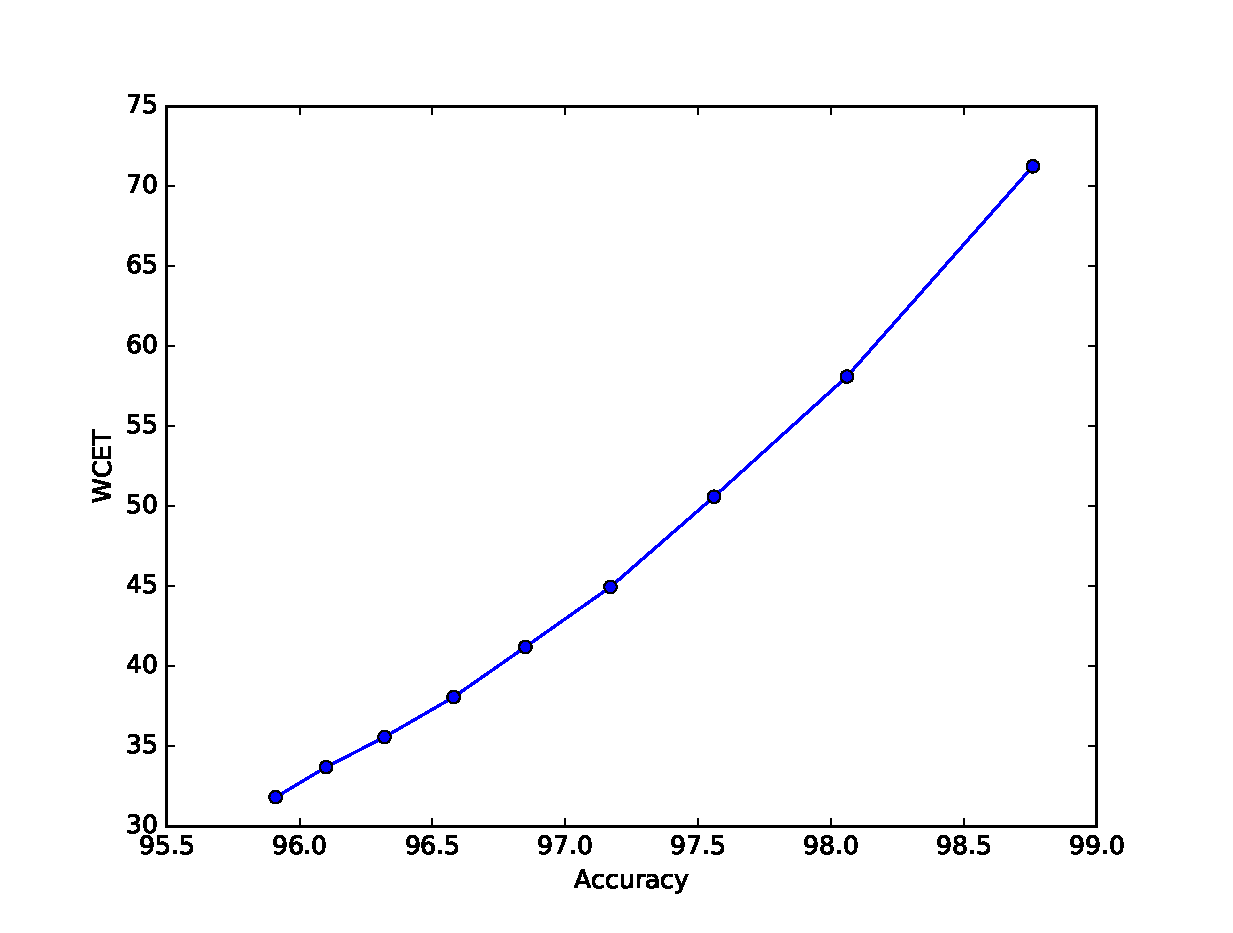
\includegraphics[width=0.95\linewidth]{Results/prime3.eps}
  \caption{WCET vs Accuracy}
  \label{prime3}
\end{figure}


\begin{enumerate}
\item The accuracy decreases as the multiplier increases. But the decrease in accuracy is slow. The relation is not linear. In a separate experiment with a multiplier of 100000, it was observed that accuracy bottoms out at 55\%. The key here is that the decrease in accuracy is slow.
\item The relation between WCET and multiplier is similar to the relation between accuracy and multiplier. The key difference is that the change in WCET is much higher than the change in the accuracy.
\item Figure \ref{prime3} shows the accuracy and WCET. Looking at the values on the axis we can clearly see that the approximation can be helpful for this benchmark since the WCET decrease to a third with just 4\% loss in accuracy. Once again, a system designer can chose the approximate version in order to satisfy deadline if the use is not critical.
\end{enumerate}


%% \begin{figure}
%%   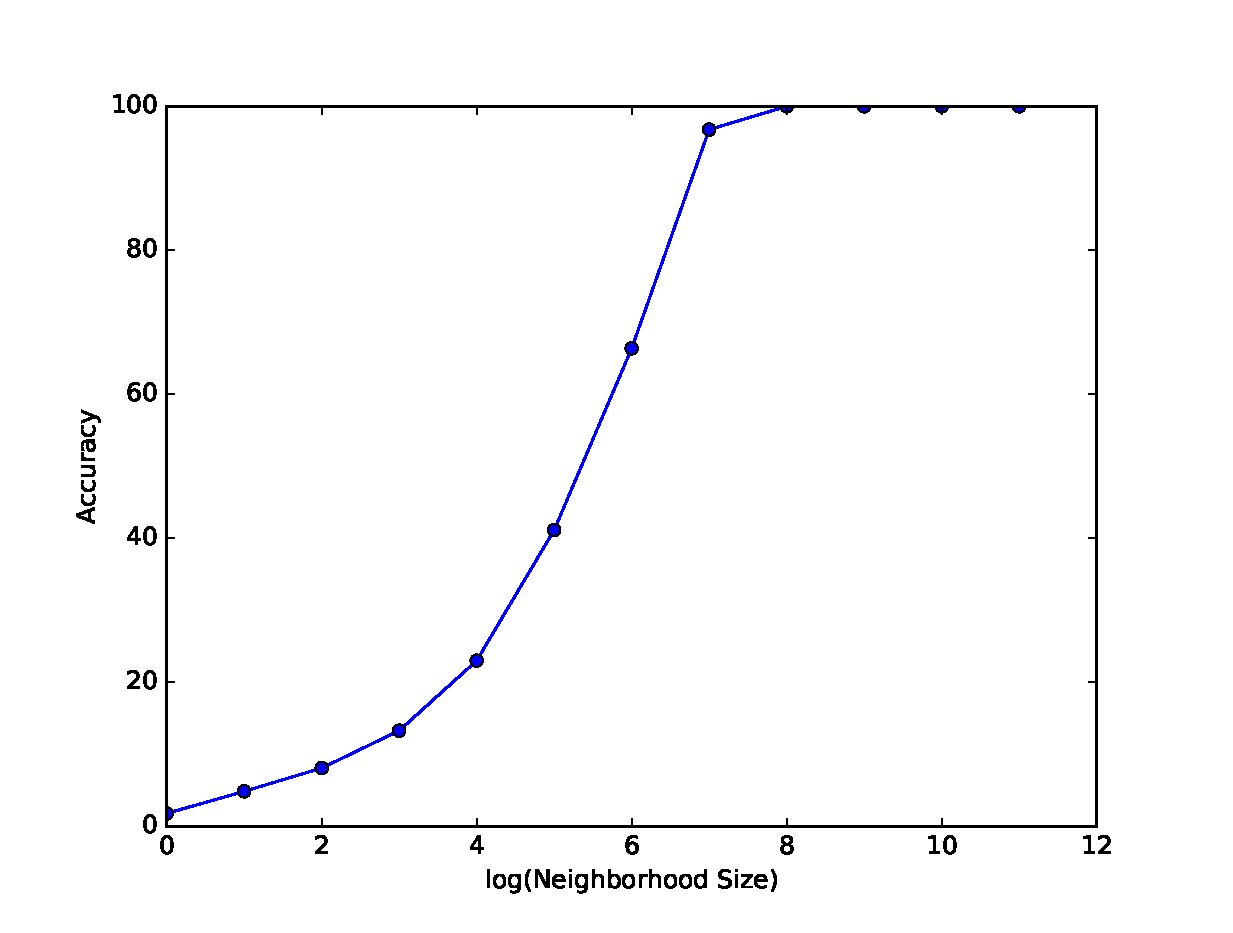
\includegraphics[width=0.95\linewidth]{Results/binarysearch1.eps}
%%   \caption{WCET vs Skipped Iterations)}
%%   \label{binarysearch2}
%% \end{figure}

